\section{Algorithmic Improvements}
\label{sec:alg_improvements}

Beyond the trust region formulation, we introduce several algorithmic improvements.
An overview is provided in \cref{alg:tr_mpc}, where the additional steps are highlighted in {\color{myblue}blue}.
Among these, the sampling method is a central design choice: we use random sampling as a baseline and introduce low-discrepancy and deterministic \ac{LCD}-based sampling as an extension.
% We therefore include both variants and compare them in \cref{sec:evaluation}.

\begin{algorithm}[t]
    \small
    \caption{Trust Region MPC Step}
    \label{alg:tr_mpc} 
    \SetKwFunction{FMain}{TR-MPC-Step}
    \SetKwInOut{Input}{Input}
    \Input{%
        State $\vx_k$, initial parameters $\paramCEM_0 = (\evVarCem_0, \mC_0)$, {\color{myblue} buffered samples from previous step}
    }%
    \SetKwInOut{Output}{Optimal control input $\vu_k^*$}
    {\color{myblue} Warm start last proposal mean and buffered samples}\;
    \For{$j \gets 0$ \KwTo $\numCEMIter-1$}{
        % Sample $\{\vVarCem^{(i)}\}_{i=1}^{\numCEMSamples} \sim \cemPropPdf(\cdot; \paramCEM_j)$\;
        Sample $\vu^{(1)}_{k:k+\horizon-1}, \ldots, \vu^{(\numCEMSamples)}_{k:k+\horizon-1} \sim \pdf(\cdot; \paramCEM_j)$\; \label{alg:tr_mpc:sampling_step}
        {\color{myblue} Add saved samples from buffer}\;
        {\color{myblue} Clip samples to input bounds}\;
        Trajectory shooting using \cref{eq:system_dynamics}\tcp*{\small \tt parallel}
        Evaluate costs $\{J_k(\vu^{(i)}_{k:k+\horizon-1})\}_{i=1}^{\numCEMSamples}$ using~\cref{eq:ocp_cost}\tcp*{\tt\small parallel}
        Solve dual problem~\cref{eq:tr_dual:opt_problem}\;
        Update proposal parameters $\paramCEM_{j+1}$ (weighted sample mean and covariance) using \cref{eq:tr_dual:weights} \;
        {\color{myblue} Add $\bufferSize$ best samples to buffer}\;
    }
    \Return first control $\vu_k^*$ from best sampled sequence
\end{algorithm}

\subsection{Sampling Methods}
\label{sec:alg_improvements:lcd_samples}
We propose to use deterministic samples based on \acp{LCD}~\cite{CDC09_HanebeckHuber} to represent the isotropic standard normal distribution $\mathcal{N}(\vVarCem;\vzero,\mI)$ optimally with a fixed number of samples. 
The optimization is done \emph{offline}, and these samples are stored for use in optimization iterations. 
For this, we use our Python package\footnote{\url{https://github.com/KIT-ISAS/deterministic_gaussian_sampling_py}}.

At each iteration $j$ the stored samples are mapped to match the proposal parameters $\paramCEM_j=(\evVarCem_j,\mC_j)$ via
\begin{align}
    \label{eq:lcd_sample_transform}
    \vVarCem_j^{(i)} = \evVarCem_j + \mL_j \, \mR_j \, \vVarLcd_{\mathrm{SN}}^{(i)} \enspace,
\end{align}
where $\mL_j$ satisfies $\mC_j=\mL_j\mL_j\T$. 
A random rotation matrix $\mR_j$ is drawn at each iteration from the special orthogonal group $SO(\dimVarCem)$ (orthogonal matrices with determinant $+1$)~\cite{leonStatisticalModelRandom2006}. 
Applying the rotation before scaling preserves the optimality because the standard normal distribution is rotationally invariant, while the random rotation introduces stochasticity that improves exploration~\cite{walkerSampleefficientSmoothCrossentropy2026}.
% Benefits of this approach include a low-discrepancy coverage of the proposal distribution for a given number of samples. Rotating the deterministic set each iteration balances exploitation of the proposal mean and covariance with exploration across directions. 
\Cref{fig:lcd_samples} illustrates the precomputed sample set and the transformation.

As alternatives, we also consider scrambled (randomized) low-discrepancy sampling using Sobol~\cite{joeConstructingSobolSequences2008} and Halton~\cite{owen2017randomizedhaltonalgorithmr} sequences, as well as standard random sampling.
Note that the root mean square error of random sampling for approximating expectations (integration) decreases proportionally to $\numCEMSamples^{-\frac{1}{2}}$, while low-discrepancy sampling scales proportionally to $(\log \numCEMSamples)^{\dimVarCem}\numCEMSamples^{-1}$~\cite{Dick2013_HighDimensionalIntegrationTheQuasiMonteCarloWay}.

In comparison to low-discrepancy sampling, \ac{LCD}-based sampling has the advantage of allowing deterministic samples to be optimized directly for Gaussians. 
In contrast, low-discrepancy sampling, such as Halton and Sobol, requires a transformation from a uniform distribution to a Gaussian distribution, which can introduce additional error and complexity.

\begin{figure}[t]
    \centering
    \begin{subfigure}{0.49\columnwidth}
        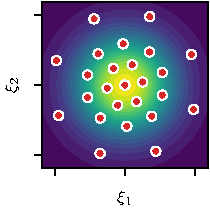
\includegraphics{images/lcd_samples/standard_normal_lcd_samples.pdf}%
        \caption{Standard normal samples}%
        \label{fig:lcd_samples:standard}%
    \end{subfigure}
    \begin{subfigure}{0.49\columnwidth}
        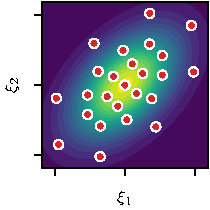
\includegraphics{images/lcd_samples/transformed_lcd_samples.pdf}%
        \caption{Transformed samples}%
        \label{fig:lcd_samples:transformed}%
    \end{subfigure}%
    \caption{Example showing \num{25} two-dimensional deterministic samples, where the \ac{PDF} is indicated by the background color (adapted  from~\cite{walkerSampleefficientSmoothCrossentropy2026}.)}%
    \label{fig:lcd_samples}%
\end{figure}


\subsection{Standard Improvements}
\label{sec:standard_improvements}

Besides sampling methods, we apply several standard enhancements commonly used in sampling-based \ac{MPC}.
We use warm starting by initializing the proposal mean at iteration $j = 0$ with the shifted mean from the previous time step, in which the last control input is duplicated to fill the horizon.
%
To enforce control input bounds, sampled controls are clipped to the admissible range. This can be viewed as modified system dynamics incorporating an additional saturation nonlinearity~\cite{williamsInformationtheoretic2018}.

We further use a buffer of size $\bufferSize$ that retains the $\bufferSize$ best trajectories (cost-based ranking) from the previous iteration, as in~\cite{walkerSampleefficientSmoothCrossentropy2026,arXiv26_Walker_IFAC}, to improve sample efficiency. 
% Note that the added samples replace existing ones to maintain a fixed buffer size.
% Note that the cache from the previous iteration is overwritten to maintain a fixed cache size.
As with the mean of the proposal, the buffered samples are also warm-started in iteration $j = 0$ in the same way as described above.

Finally, to encourage smooth control trajectories, we use a time-correlated proposal covariance.
The time-correlation structure is derived from colored noise with power spectral density $\mathrm{PSD}(\omega) \propto \nicefrac{1}{\omega^{\beta}}$, where $\beta$ controls the noise color and $\omega$ denotes frequency. Within a time step, the controls are assumed to be uncorrelated.
During optimization, only marginal variances are updated, while the correlation structure is kept fixed, since estimating full covariance matrices from a few samples is error-prone.
Further details are provided in~\cite{arXiv26_Walker_IFAC}.